\chapter{Introduction}
\label{chap:Introduction}

%% Restart the numbering to make sure that this is definitely page #1!
\pagenumbering{arabic}

The field of neutrino physics is currently evolving very rapidly.  With its tenuous postulation~\cite{PauliOpenLetter} acting as a future omen, the neutrino's mark on history would not become apparent from its discovery~\cite{Cowan20071956, PhysRevLett.9.36, Kodama2001218}, but rather from a spate of surprising discoveries at the end of the 20th century~\cite{PhysRevLett.81.1562, PhysRevLett.87.071301, PhysRevLett.90.021802} which conclusively proved that the Standard Model, while very successful, was incomplete.  This revelation was experimental proof of Maki, Nagakawa and Sakata's extension~\cite{Maki01111962} to Pontecorvo's theory of neutrino oscillation\Yoshi{}{ADDRESSED - there was a space here}~\cite{Pontecorvo} \Yoshi{with the inclusion of the Mikheyev-Smirnov-Wolfenstein (MSW) effect which is the alteration of the oscillation effect due to differences in the coherent forward scattering of the three neutrino flavours with electrons in matter}{ADDRESSED - this is not very clear. Add a few words to remind readers of what the MSW effect is.}~\cite{PhysRevD.17.2369,Mikheev:1986gs}.  The findings were ground breaking as the underlying theory requires \Yoshi{neutrinos to be massive}{ADDRESSED - massive neutrinos}, which is in direct contradiction to the Standard Model.  The, now, standard theory of neutrino oscillation defines three neutrino flavours and three neutrino masses.  However, the map between flavour and mass is not one-to-one, but rather a rotation of mass space onto flavour space.  The main consequence of this rotation is that the flavour eigenstates are a superposition of mass eigenstates, namely
\begin{equation}
\ket{\nu_\alpha} = \sum^{3}_{i=k}U^{\ast}_{\alpha k}\ket{\nu_k},
\label{eq:NeutrinoEigenstates}
\end{equation}
where $\alpha \in \{e,\mu, \tau\}$, $\nu_k$ are the neutrino mass eigenstates and $U^{\ast}_{\alpha k}$ is an element of a unitary rotation matrix which is known as the PMNS mixing matrix.  As there are \Yoshi{three}{ADDRESSED - was 3 (house style to spell out numbers below 10)} mass and flavour eigenstates, the PMNS matrix is a $3\times3$ matrix and is often parameterised as 
\begin{equation}
U \equiv
\begin{pmatrix}
1 & 0 & 0 \\
0 & c_{23} & s_{23} \\
3 & -s_{23} & c_{23}
\end{pmatrix}
\begin{pmatrix}
c_{13} & 0 & s_{13}e^{-i\delta} \\
0 & 1 & 0 \\
-s_{13}e^{i\delta} & 0 & c_{13} 
\end{pmatrix}
\begin{pmatrix}
c_{12} & s_{12} & 0 \\
-s_{12} & c_{12} & 0 \\
0 & 0 & 1
\end{pmatrix}
,
\label{eq:PMNSMatrix}
\end{equation}
where $c_{ij} \equiv \cos\theta_{ij}$ and $s_{ij} \equiv \sin\theta_{ij}$. $\theta_{ij}$ are known as the mixing angles \Yoshi{and}{ADDRESSED - was which} parametrise how strong mixings between the flavour and mass eigenstates are\Yoshi{,}{ADDRESSED - comma} and $\delta$ is a CP violating phase.  The most surprising observable feature of this mechanism is the non-zero probability to detect a neutrino of specific flavour which was created at source in a different flavour state.  By propagating the mass eigenstates through time, one can arrive at this probability which has the following form\Yoshi{:}{ADDRESSED - ``has the following form'' needs a colon; ``has the form'' does not}
\begin{equation}
P(\nu_\alpha \rightarrow \nu_\beta) = |\braket{\nu_\beta|\nu\left(t\right)}|^2 = |U_{\beta k} e^{-iE_{k}t}  U^{\ast}_{\alpha k}|^2,
\label{eq:NeutrinoOscillationProbability}
\end{equation}
where $\nu\left(t\right)$ is the time-dependent neutrino mass eigenstate and $E_k$ is the energy of the $\nu_k$.  For an accelerator-based neutrino oscillation experiment, the beam will be $\nu_\mu$\Yoshi{-}{ADDRESSED - hyphen}dominated.  So, the $\nu_\mu$ survival probability, $P(\nu_\mu \rightarrow \nu_\mu)$, and $\nu_e$ appearance probability, $P(\nu_\mu \rightarrow \nu_e)$, which are typically of interest, can be approximated in the following forms\Yoshi{:}{ADDRESSED - }
\begin{equation}
  \Yoshi{P(\nu_\mu \rightarrow \nu_\mu) \approx 1 - \cos^{4}\theta_{13}\sin^{2}2\theta_{23}\sin^2\left(1.27\frac{\Delta m^{2}_{23}}{\left[\textrm{eV}^2\right]}\frac{L}{\left[\textrm{km}\right]}\frac{\left[\textrm{GeV}\right]}{E}\right)}{ADDRESSED - would units not be in square brackets?}
  \label{eq:MuonNeutrinoSurvivalProbability}
\end{equation}
\begin{equation}
  \Yoshi{P(\nu_\mu \rightarrow \nu_\mu) \approx \sin^{2}2\theta_{13}\sin^{2}\theta_{23}\sin^2\left(1.27\frac{\Delta m^{2}_{23}}{\left[\textrm{eV}^2\right]}\frac{L}{\left[\textrm{km}\right]}\frac{\left[\textrm{GeV}\right]}{E}\right),}{ADDRESSED - would units not be in square brackets?}
  \label{eq:ElectronNeutrinoAppearanceProbability}
\end{equation}
where $\Delta m^{2}_{ij} \equiv m^{2}_{i} - m^{2}_{j}$, $L$ is the distance the neutrino propagates and $E$ is the energy of the neutrino.

\section{The state of the field}
\label{sec:StateOfTheField}
Data provided from a wide range of experiments show excellent agreement with the theory of neutrino oscillation and with a \Yoshi{ADDRESSED - three-}{was ``3''}flavour neutrino picture.  Global fits applied to the data provided by these experiments gives best fit values for the oscillation parameters, which are summarised in table~\ref{table:NeutrinoOscillationParameterValues}~\cite{Agashe:2014kda}.  The experiments which provided the data inputs to the global fit generally fall into one of four categories, with each category sensitive to a different subset of the neutrino oscillation parameters.
\begin{table}
  \begin{tabular}{l c }
    Parameter & best-fit $(\pm1\sigma)$ \\ \hline \hline
    $\Delta m^2_{12}$ [$10^{-5}\textrm{eV}^2$] & $7.54^{+0.26}_{-0.22}$ \\
    $|\Delta m^2|$ [$10^{-3}\textrm{eV}^2$] & $2.43\pm0.06$ $(2.36\pm0.06)$ \\
    $\sin^2\theta_{12}$ & $0.308\pm0.017$ \\
    $\sin^2\theta_{23}$, $\Delta m^2 > 0$ & $0.437^{+0.033}_{-0.023}$ \\
    $\sin^2\theta_{23}$, $\Delta m^2 < 0$ & $0.455^{+0.039}_{-0.031}$ \\
    $\sin^2\theta_{13}$, $\Delta m^2 > 0$ & $0.0234^{+0.0020}_{-0.0019}$ \\
    $\sin^2\theta_{13}$, $\Delta m^2 < 0$ & $0.0240^{+0.019}_{-0.022}$ \\
    $\sin^2\theta_{13}$, $\Delta m^2 < 0$ & $0.0240^{+0.019}_{-0.022}$ \\
    $\delta/\pi$ ($2\sigma$ range quoted) & $1.39^{+0.38}_{-0.27}$ $(1.31^{+0.29}_{-0.33})$ \\
  \end{tabular}
  \caption{The 2014 best-fit values of the 3-neutrino oscillation parameters provided by the Particle Data Group~\cite{Agashe:2014kda}. $\Delta m^2 \equiv m^2_3 - \left(m^2_2 - m^2_1\right)/2$. The values (values in brackets) correspond to $m_1 < m_2 < m_3$ ($m_3 < m_1 < m_2$).  \Yoshi{The values come from a global fit to solar, atmospheric, reactor and accelerator (both short and long baseline) experiments~\cite{PhysRevD.89.093018}.  The most recent contributing data is a precision measurement of $\nu_\mu$ disappearance from T2K (2014)~\cite{PhysRevLett.112.181801}}{ADDRESSED - Say when these numbers come from (year and month), and perhaps the most recent experiments that contributed}.}
  \label{table:NeutrinoOscillationParameterValues}
\end{table}
\newline
\newline
Reactor neutrino experiments measure $\bar{\nu}_e$ disappearance provided by inverse $\beta$ decay in nuclear reactors with an average neutrino energy of 3~MeV.  The baseline for oscillations varies between experiments, but a baseline of around 1~km provides excellent sensitivity to $\theta_{13}$. Examples of reactor experiments are Double CHOOZ~\cite{Abe201366}, Daya Bay~\cite{PhysRevLett.108.171803} and RENO~\cite{PhysRevLett.108.191802}.
\newline
\newline
Solar neutrino experiments detect neutrinos generated in the core of the Sun as a result of nuclear \Yoshi{fusion}{ADDRESSED -} reaction chains.  Such experiments are primarily sensitive to $\theta_{12}$ and $\Delta m^{2}_{12}$\Yoshi{,}{ADDRESSED -} which are often referred to as the solar mixing parameters.  The final\Yoshi{-}{ADDRESSED -}state neutrinos created in the Sun's core are MeV-scale $\nu_e$ but, because of propagation through the core's surrounding matter, the MSW effect results in a highly\Yoshi{-}{ADDRESSED -}pure state of $\nu_2$ at the Sun's surface.  As $\nu_2$ is a mass eigenstate, no oscillation occurs between the surface of the Sun and the Earth.  Homestake~\cite{0004-637X-496-1-505}, SAGE~\cite{PhysRevC.80.015807} and SNO~\cite{PhysRevLett.87.071301} are examples of such experiments.  It should be noted here that the KamLAND experiment~\cite{PhysRevLett.90.021802}, while a reactor neutrino experiment, was sensitive to the solar mixing parameters due to its 180~km baseline.
\Yoshi{}{ADDRESSED - FIXME: You should mention KamLAND, which sees 1-2 oscillations in vacuum, not requiring the matter effect.}
\newline
\newline
Atmospheric neutrino experiments detect neutrinos which are produced when $\pi$ and $K$ mesons, created by cosmic rays interactions with the upper atmosphere of the Earth, decay.  The neutrinos produced are a mixture of $\nu_\mu$, $\bar{\nu}_\mu$, $\nu_e$ and $\bar{\nu}_e$.  Because the cosmic ray flux is fairly uniform, atmospheric neutrino experiments are exposed to neutrinos from all directions, which results in a very wide range of oscillation baselines.  The oscillation parameters that such experiments are sensitive to are $\theta_{23}$ and $\Delta m^2_{13}$. Super-Kamiokande~\cite{PhysRevLett.81.1562} is an example of an atmospheric neutrino experiment. 
\newline
\newline
\Yoshi{Long-baseline a}{ADDRESSED - I think the paragraph excludes short-baseline experiments}ccelerator neutrino experiments produce beams of high purity $\nu_\mu$ (or $\bar{\nu}_\mu$) at GeV-scale energy with wide\Yoshi{-}{ADDRESSED - hyphen}ranging baselines which are generally $\mathcal{O}\left(100~\textrm{km}\right)$.  The highly man-made nature of such experiments allows almost complete control over $L/E$ allowing careful tuning of parameter sensitivity.  Accelerator neutrino experiments are generally sensitive to $\theta_{13}$, $\theta_{23}$, $\Delta m^{2}_{13}$ and $\delta$. K2K~\cite{PhysRevD.74.072003}, MINOS~\cite{PhysRevLett.97.191801}, T2K~\cite{PhysRevLett.112.061802} and NO$\nu$A~\cite{Ayres:2004js}are examples of such experiments.

\section{The future}
\label{sec:NeutrinoFieldFuture}
It should be clear that an immense amount of progress has been made in the field, with remarkable contributions to the picture coming \Yoshi{in only}{ADDRESSED - was ``only in'', which excludes any remarkable contributions before 20 years ago. But the discovery of neutrinos and the solar neutrino problem etc. were pretty remarkable too....} the last 20 years.  However, there are several key questions which remain unanswered.  
\newline
\newline
By far the most sought\Yoshi{-}{ADDRESSED - hyphen}after answer is whether CP violation occurs in the lepton sector.  The magnitude of CP violation is encapsulated in the CP violating phase $\delta$ and so it is this parameter which current and future long-baseline experiments are aiming towards.  \Yoshi{Currently, only T2K and NO$\nu$A can provide hints for values of $\delta$, with the possibility of future constraints.}{ADDRESSED - reword this sentence -- it sounds almost as if you are saying they do provide the strongest constraints, because of the word `Currently'. Right now they just provide the only hints we have and if we are lucky they will be able to provide constraints, perhaps} The future long-baseline experiments, Hyper-Kamiokande~\cite{Abe:2014oxa} and DUNE (formerly LBNE)~\cite{Adams:2013qkq} are being designed with a possible measurement of $\delta$ as a primary goal.
\newline
\newline
The second question still to be answered is the ordering of the mass eigenstates.  \Yoshi{It is not known whether $\nu_1$, which is dominated by the electron neutrino, or $\nu_3$ is the lightest mass eigenstate.}{ADDRESSED - you need something here}  Written more succinctly, is $m_3 \gg m_2 > m_1$ (the normal mass hierarchy) or $m_2 > m_1 \gg m_3$ (the inverted mass hierarchy)?  This is known as the mass hierarchy problem and its two possible solutions are shown in Fig.~\ref{fig:MassHierarchy}.  The matter effects introduced by the MSW effect are mass hierarchy\Yoshi{-}{ADDRESSED - hyphen}dependent.  So, for very long-baseline experiments, there is mass hierarchy sensitivity.  Currently NO$\nu$A has \Yoshi{the potential to resolve}{ADDRESSED - set to resolve is too strong} the mass hierarchy problem.  However, both Hyper-Kamiokande (via atmospheric measurements) and DUNE have measurement of the mass hierarchy as a primary goal.
\begin{figure}%
  \centering
  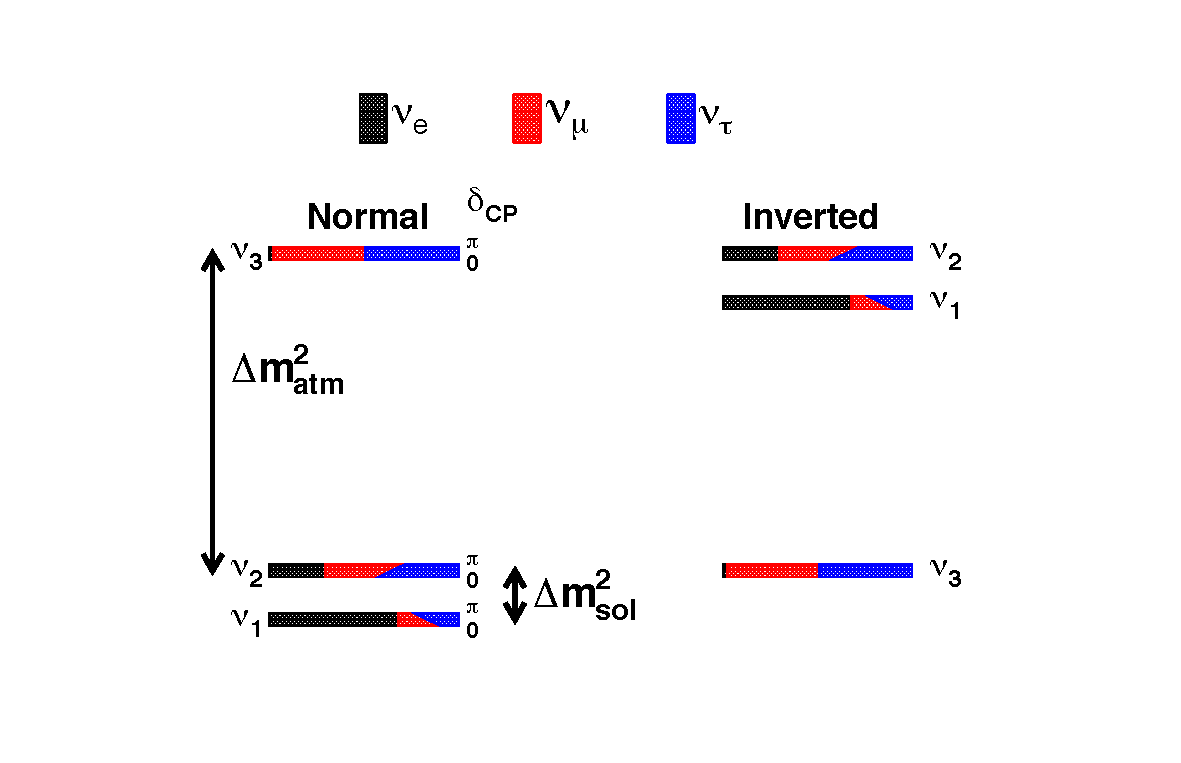
\includegraphics[width=10cm]{images/introduction/mass_hierarchy.pdf}
  \caption{The pattern of neutrino masses for the normal and inverted hierarchies with the atmospheric ($\Delta \textrm{m}^2_{\textrm{atm}}$) and solar ($\Delta \textrm{m}^2_{\textrm{sol}}$) mass splittings labelled.  The flavour composition of the mass eigenstates as a function of the unknown CP phase (labelled $\textrm{\delta}_{\textrm{CP}}$) is also shown~\cite{Qian20151}.}
  \label{fig:MassHierarchy}
\end{figure}
\newline
\newline
Oscillation experiments only have the capability to measure the \Yoshi{differences between the square of the neutrino masses}{ADDRESSED - Careful with language: was square of the mass splitting differences}.  This means that all oscillation experiments have no sensitivity to the absolute neutrino mass scale and an entirely different type of neutrino experiment is required.  Neutrinos are one of the final states associated with $\beta$ decay and the mass of the neutrino should appear as a cut off in the $\beta$ spectrum.  The visibility of the cut-off entirely depends on the mass scale.  So, the KATRIN experiment~\cite{Weinheimer2002141} will attempt to utilise \Yoshi{this feature of $\beta$ decay}{ADDRESSED - awkward. Reword.}, with a neutrino mass sensitivity of $0.2$~eV.
\newline
\newline
It is not currently known whether neutrinos are their own anti-particle, \Yoshi{which are referred to as}{ADDRESSED - you're omitting some of the logic of the sentence} Majorana neutrinos.  \Yoshi{A widely accepted method of studying the Majorana neutrino hypothesis is neutrinoless double $\beta$ decay in which a pair of neutrons in a nucleus undergo $\beta$ decay with the final state neutrinos pair-annihilating due to their Majorana nature.  A large neutrinoless double $\beta$ decay experiment effort is ongoing, including EXO~\cite{PhysRevLett.109.032505}, SuperNEMO~\cite{1742-6596-375-4-042012} and SNO+~\cite{Chen:2008un}}{ADDRESSED - a bit redundant --- reword more carefully, with more specificity}.
\newline
\newline
The short-baseline neutrino oscillation programme has seen several anomalies~\cite{ShortBaseLineAnomaly} which remain unexplained.  The LSND experiment found evidence of $\bar{\nu}_e$ in a $\bar{\nu}_\mu$ beam, which was consistent with neutrino oscillations~\cite{Aguilar:2001ty}.  However the data suggested a mass-squared splitting of 0.2\Yoshi{--}{ADDRESSED - an en-dash '--' for ranges, not a hyphen '-'}10~eV$^2$.  This large splitting is consistent with a fourth species of neutrino.  Because the data suggesting \Yoshi{three}{ADDRESSED - was 3} flavours of weakly-interacting neutrino is strong\Yoshi{\cite{Z-PeakReferenceAtLEP}}{ADDRESSED - Z-peak measurement at LEP reference}, this postulated fourth species must not interact through the weak force, and are generally referred to as \Yoshi{sterile neutrinos}{ADDRESSED - define `sterile' (it is neutrino-area jargon}.  More recently, the MiniBooNE experiment observed a \Yoshi{separate}{ADDRESSED - not similar, actually --- read carefully about what MiniBooNE says about LSND-oscillations} short\Yoshi{-}{ADDRESSED - hyphen}baseline excess of $\bar{\nu}_e$ in a $\bar{\nu}_\mu$ beam with a mass-squared splitting of 0.01-1.0~eV$^2$~\cite{Aguilar-Arevalo:2013pmq}, further suggesting the sterile hypothesis.  New experiments are now under development which aim to test this hypothesis, which include MicroBooNE~\cite{2011arXiv1110.1604I} and SBND (formally LAr1-ND)~\cite{Adams:2013uaa}.

\Yoshi{}{ADDRESSED - A general comment would be that I don't get a sense of the variety of regions that are involved in these experiments---because you don't say things like ``...at Fermilab''. If this is a conscious choice, that is fine....}
